\documentclass{article}

% NeurIPS 2026 style
\usepackage[final]{neurips_2026}

\usepackage[utf8]{inputenc}
\usepackage[T1]{fontenc}
\usepackage{hyperref}
\usepackage{url}
\usepackage{booktabs}
\usepackage{amsfonts}
\usepackage{amsmath}
\usepackage{nicefrac}
\usepackage{microtype}
\usepackage{graphicx}
\usepackage{xcolor}
\usepackage{algorithm}
\usepackage{algorithmic}
\usepackage{subcaption}
\usepackage{wrapfig}
\usepackage{multirow}
\usepackage{listings}

\newtheorem{proposition}{Proposition}

% Python code style matching Kimi paper (Figure 2)
\lstdefinestyle{python}{
  language=Python,
  basicstyle=\ttfamily\small,
  keywordstyle=\color[rgb]{0.0,0.5,0.0}\bfseries,
  stringstyle=\color[rgb]{0.75,0.0,0.0},
  commentstyle=\color[rgb]{0.5,0.5,0.5}\itshape,
  numberstyle=\tiny\color{gray},
  numbers=left,
  numbersep=6pt,
  xleftmargin=2em,
  framexleftmargin=1.5em,
  breaklines=true,
  showstringspaces=false,
  tabsize=4,
  columns=fullflexible,
  keepspaces=true,
  morekeywords={Tensor, Linear, RMSNorm, list, tuple, self, None},
}

\title{Delta Attention Residuals: Source Representation and Per-Stream Routing for Cross-Layer Information Flow}

\author{
  Cheng Luo \\
  \texttt{wdlctc@gmail.com} \\
  \And
  Zefan Cai \\
  \texttt{zefan.czf@gmail.com} \\
}

\begin{document}

\maketitle

\begin{abstract}
Attention Residuals~\citep{kimi2025attention} replace standard additive residual connections with learned softmax attention over previous layer outputs, enabling selective cross-layer information routing. We identify two overlooked design dimensions that substantially impact routing effectiveness. \textbf{(1)~What to route}: attending over per-sublayer outputs (``deltas'') rather than cumulative hidden states reduces WikiText-2 perplexity by 19.2\% relative to cumulative-state AttnRes and 7.5\% relative to the baseline, because cumulative states exhibit 0.95 cosine similarity that collapses softmax routing. \textbf{(2)~Where to route}: giving the value stream its own independent depth-routing query---separate from query/key---provides additional gains on top of both delta and cumulative sources. These two dimensions are \emph{orthogonal and composable}: combining delta sources with per-stream V-routing achieves the best results across all configurations, reducing validation loss by 3.0\% over the baseline on nanoGPT Shakespeare benchmarks. Delta AttnRes's additive formulation also enables effective fine-tuning of pretrained models, achieving 29.2\% PPL reduction on Qwen3-0.6B. We release code, pretrained weights, and visualization tools at \url{https://github.com/wdlctc/open-attention-residuals}.
\end{abstract}

%% ============================================================
\section{Introduction}
%% ============================================================

Residual connections~\citep{he2016deep} are fundamental to training deep transformers~\citep{vaswani2017attention}. The standard update $h_l = h_{l-1} + f_{l-1}(h_{l-1})$ accumulates all sublayer outputs with fixed unit coefficients, providing gradient highways~\citep{veit2016residual} but no selectivity over the depth dimension. This uniform aggregation persists in modern architectures from GPT-2~\citep{radford2019gpt2} to Llama~\citep{touvron2023llama}. Attention Residuals~\citep{kimi2025attention} address this by replacing fixed aggregation with learned softmax attention over previous outputs, achieving improved scaling laws~\citep{kaplan2020scaling} at up to 16B parameters.

Yet the design space of Attention Residuals remains underexplored along two dimensions: \emph{what to route} (the source representation) and \emph{where to route} (whether different information streams share the same routing). The original paper defines sources as individual sublayer outputs $v_i = f_i(h_i)$ (the ``deltas'' added at each layer), but a seemingly equivalent implementation stores cumulative hidden states $h_i = h_0 + \sum_{j=1}^{i} v_j$ instead. Meanwhile, all prior work uses a single routing decision shared across the Q, K, and V projections within each attention sublayer. We show that both choices have dramatic consequences.

\begin{figure}[t]
\centering
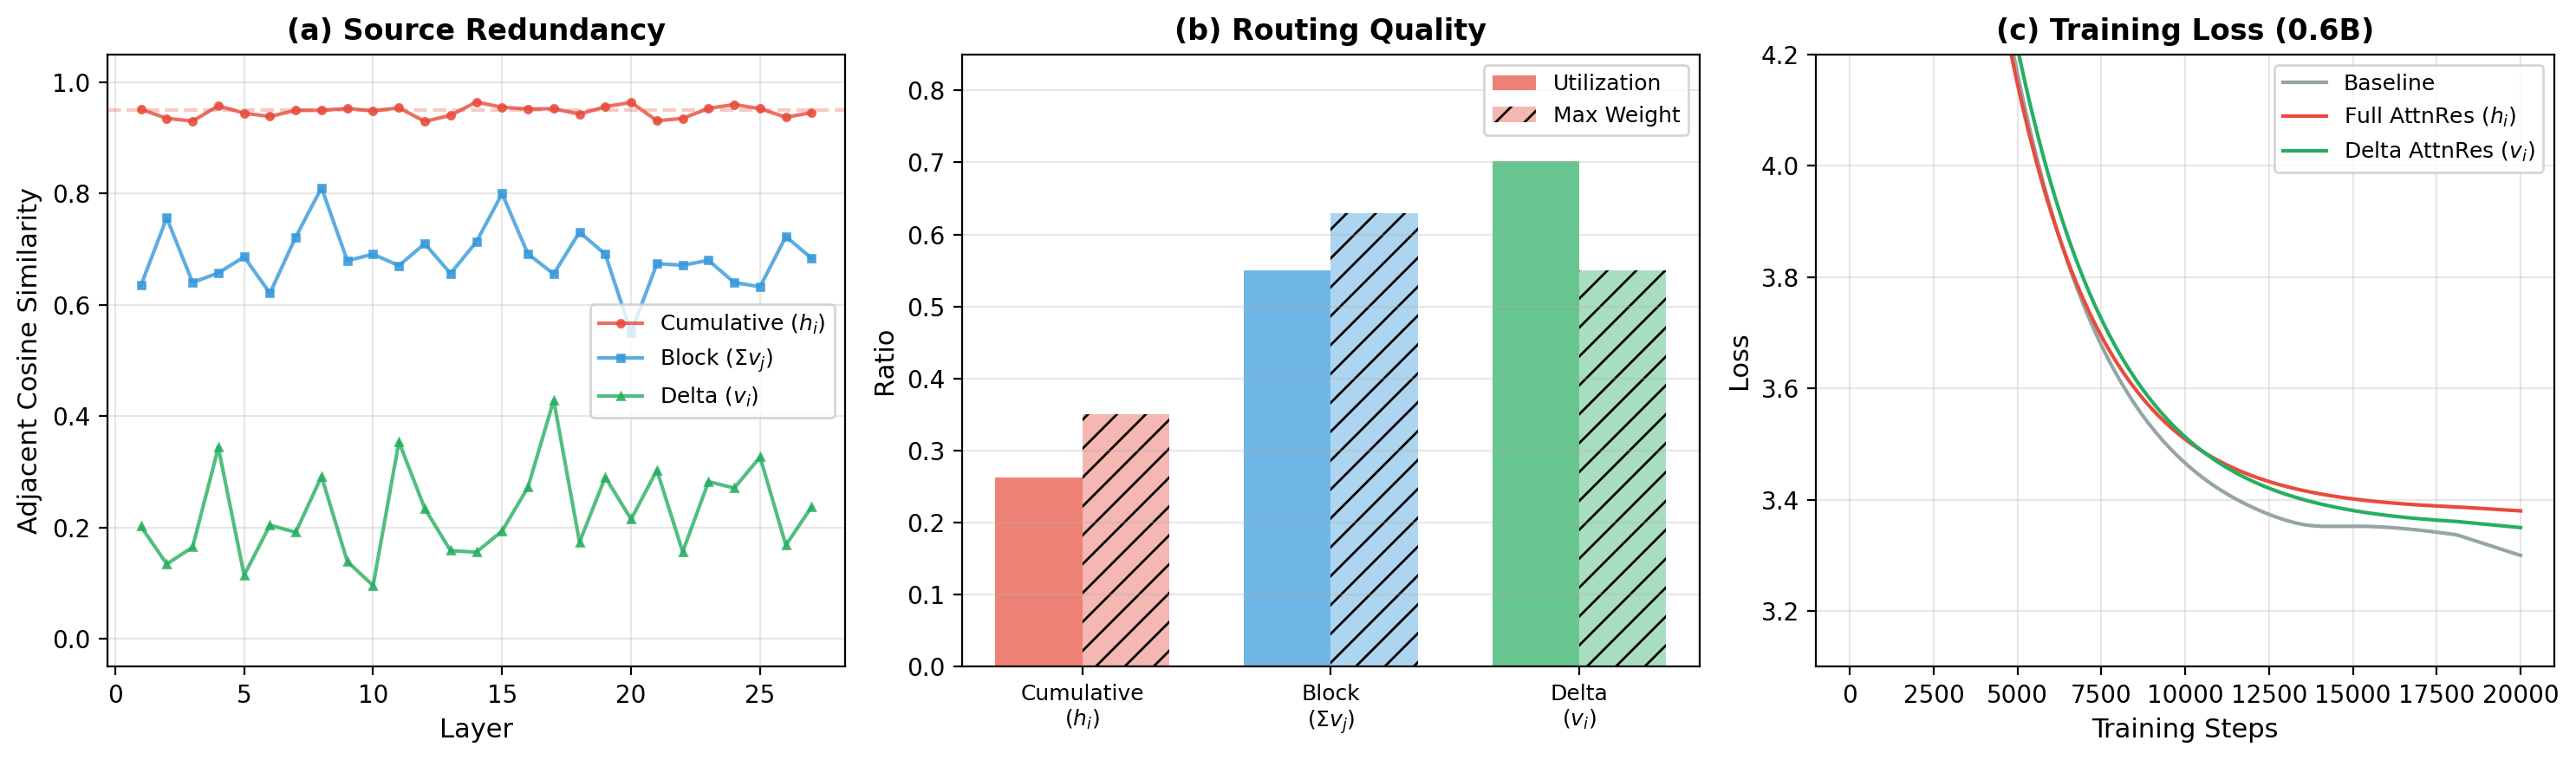
\includegraphics[width=\textwidth]{figures/fig1_delta_vs_cumulative.png}
\caption{\textbf{Source representation determines routing quality.} (a)~Cosine similarity between adjacent sources: cumulative states $\sim$0.95 (red), delta outputs $<$0.3 (green). (b)~Routing quality metrics: delta sources achieve higher utilization and sharper max weights. (c)~Training loss comparison at 0.6B scale.}
\label{fig:motivation}
\end{figure}

Our central finding is that \textbf{cumulative-state sources are degenerate for softmax routing}. Since $h_{i+1} = h_i + v_i$ and $\|v_i\| \ll \|h_i\|$ for trained models, adjacent cumulative states have cosine similarity $\sim$0.95 (Figure~\ref{fig:motivation}a). This renders the 57-way softmax nearly uniform: the effective rank drops to 15 out of 57 sources, and the maximum attention weight plateaus at 0.35. The model cannot learn selective cross-layer shortcuts because all sources look the same.

Delta sources avoid this by construction. Attention outputs and MLP outputs occupy different subspaces; outputs from different layers capture different abstraction levels. The softmax can therefore make sharp, meaningful routing decisions. At 0.6B scale, Delta AttnRes achieves WikiText-2 PPL of 55.69 compared to 68.87 for cumulative-state AttnRes and 60.21 for the standard baseline---a 19.2\% and 7.5\% reduction, respectively.

In summary, our contributions are:
\begin{enumerate}
    \item \textbf{What to route --- Delta source representation}: We identify the source redundancy problem (cumulative states have 0.95 cosine similarity) and show that attending over per-sublayer outputs (``deltas'') consistently outperforms cumulative-state variants, achieving 7.5--19.2\% PPL reduction across scales (\S\ref{sec:analysis}, \S\ref{sec:experiments}).
    \item \textbf{Where to route --- Per-stream V-routing}: We introduce independent depth routing for the value stream, decoupled from Q/K. This provides additional gains on top of \emph{both} delta and cumulative sources, adding only 0.011\% parameters (\S\ref{sec:per_stream}). The two dimensions are orthogonal and composable.
    \item We show that Delta AttnRes's \textbf{additive formulation enables effective fine-tuning} of pretrained models, achieving 29.2\% PPL reduction when fine-tuning Qwen3-0.6B (\S\ref{sec:finetune}).
    \item We provide a \textbf{systematic ablation} across the full $\{$cumulative, delta$\}$ $\times$ $\{$shared, per-stream$\}$ design space, validating on both nanoGPT (10M) and Qwen3 (100M--1.7B) architectures (\S\ref{sec:ablation}).
    \item We release an open-source implementation with code, pretrained weights, and visualization tools.\footnote{\url{https://github.com/wdlctc/open-attention-residuals}}
\end{enumerate}

%% ============================================================
\section{Delta Attention Residuals}
\label{sec:method}
%% ============================================================

\subsection{Preliminaries}

A Pre-Norm transformer~\citep{vaswani2017attention,xiong2020prenorm} with $L$ layers updates the hidden state via:
\begin{align}
    h_l^{\mathrm{mid}} &= h_{l-1} + \mathrm{Attn}(\mathrm{LN}(h_{l-1})), \label{eq:attn_update} \\
    h_l &= h_l^{\mathrm{mid}} + \mathrm{MLP}(\mathrm{LN}(h_l^{\mathrm{mid}})) \label{eq:mlp_update}
\end{align}
Writing the $i$-th sublayer output as $v_i = f_i(h_i)$, the hidden state at sublayer $l$ is $h_l = h_0 + \sum_{i=1}^{l} v_i$. All sublayer outputs are aggregated with fixed unit coefficients---no learned selectivity over depth.

Attention Residuals~\citep{kimi2025attention} replace the uniform sum with a learned weighted sum:
\begin{equation}
    \hat{h}_l = \sum_{i=0}^{l-1} \alpha_{i \to l} \cdot s_i, \quad
    \alpha_{i \to l} = \frac{\exp(w_l^\top \mathrm{RMSNorm}(s_i))}{\sum_{j=0}^{l-1} \exp(w_l^\top \mathrm{RMSNorm}(s_j))}
    \label{eq:attnres}
\end{equation}
where $s_i$ are the sources being attended over, and $w_l \in \mathbb{R}^d$ is a learned per-sublayer query initialized to zero. The critical question is: what should $s_i$ be?

\subsection{Source Representations: Cumulative vs.\ Delta}

\begin{figure}[t]
\centering
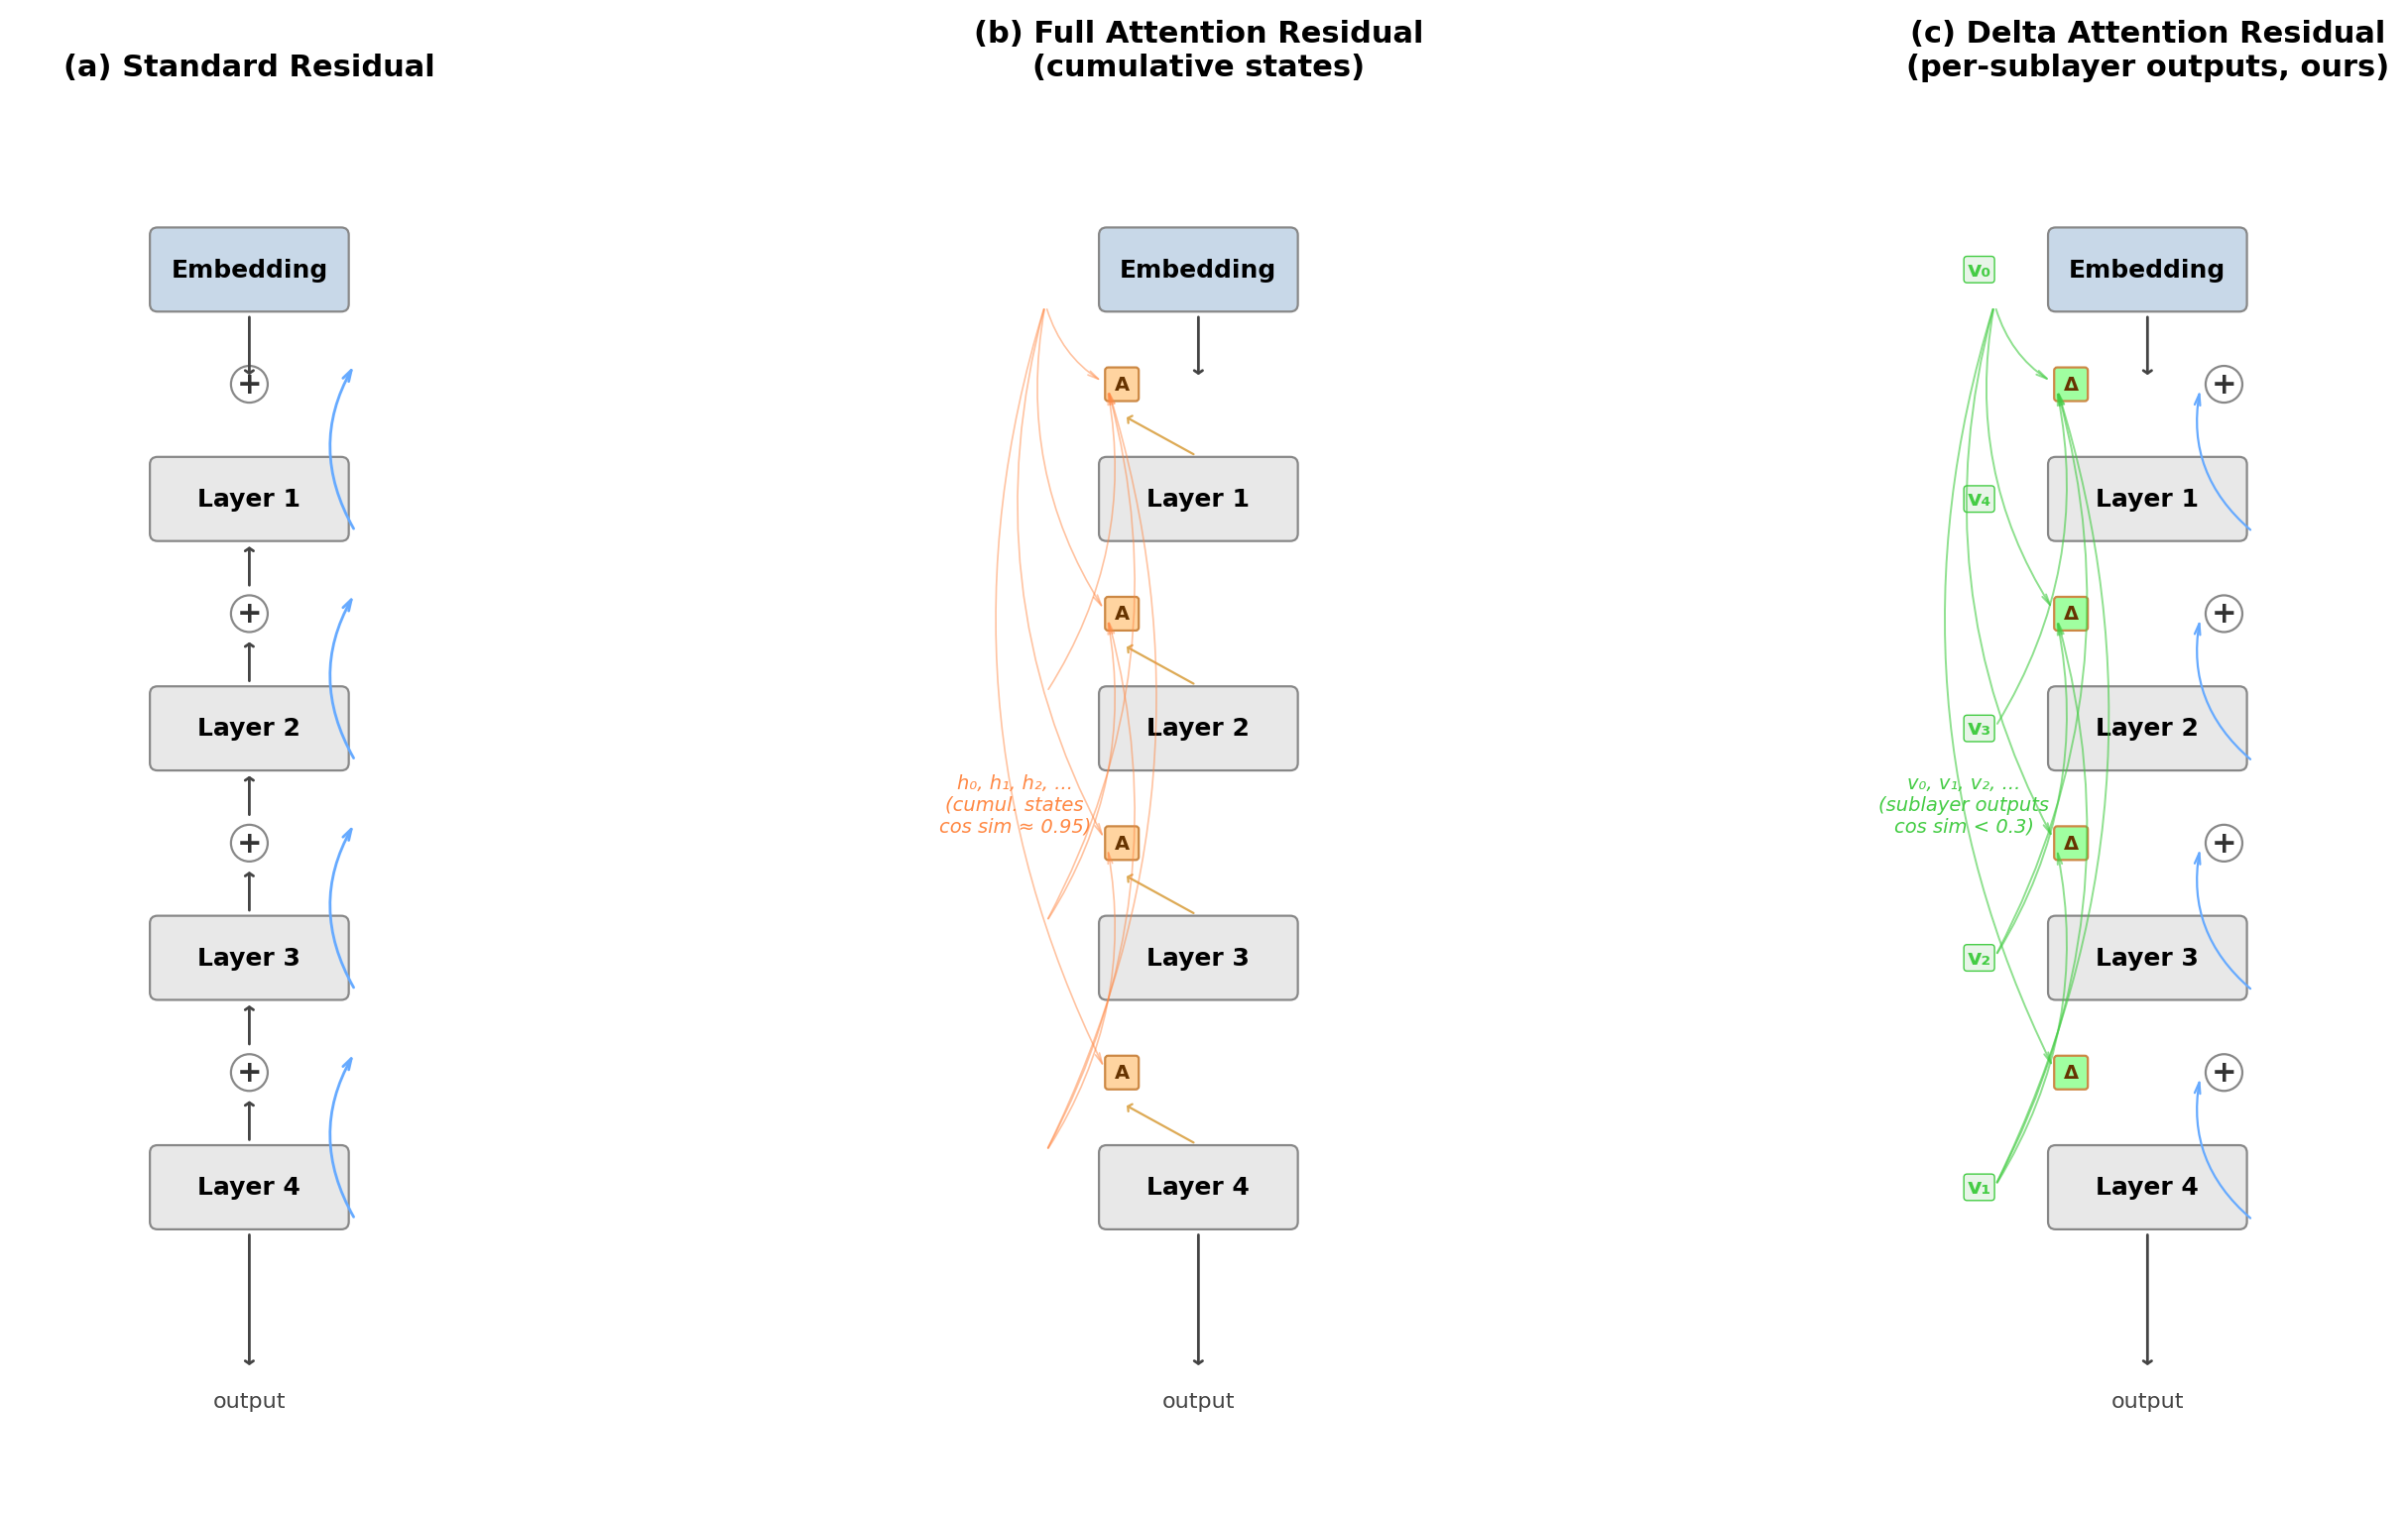
\includegraphics[width=\textwidth]{figures/fig1_architecture.png}
\caption{\textbf{Architecture comparison.} (a)~Standard residual connections uniformly add sublayer outputs. (b)~Full Attention Residuals~\citep{kimi2025attention} attend over cumulative hidden states $h_0, h_1, \ldots$, but adjacent states have cosine similarity $\sim$0.95, degrading the softmax routing. (c)~\textbf{Delta Attention Residuals (ours)} attend over individual sublayer outputs $v_0, v_1, \ldots$ (the ``deltas''), which are naturally distinctive (cos sim $<$0.3), and \emph{add} the selected information to the residual stream.}
\label{fig:architecture}
\end{figure}

We consider two source representations:

\paragraph{Cumulative sources.} $s_i = h_i = h_0 + \sum_{j=1}^{i} v_j$. Each source is the full hidden state after sublayer $i$. This is intuitive (``attend over what the model has computed so far'') and memory-efficient (hidden states are already computed). However, adjacent sources satisfy $h_{i+1} = h_i + v_i$ where $\|v_i\| \ll \|h_i\|$, causing high redundancy.

\paragraph{Delta sources.} $s_i = v_i = f_i(h_i)$ for $i \geq 1$ and $s_0 = h_0$ (embedding). Each source is the \emph{incremental contribution} of a single sublayer. Since $v_i$ is the raw output of an attention or MLP computation, sources from different sublayer types and depths are structurally diverse.

\begin{proposition}[Informal]
For a trained transformer where sublayer outputs have bounded norm $\|v_i\| \leq \epsilon \|h_i\|$ with $\epsilon \ll 1$, adjacent cumulative sources satisfy:
\begin{equation}
    \mathrm{cos}(h_i, h_{i+1}) = \frac{h_i^\top (h_i + v_i)}{\|h_i\|\|h_i + v_i\|} \geq 1 - O(\epsilon^2)
\end{equation}
Thus softmax logits $w^\top \mathrm{RMSNorm}(h_i) \approx w^\top \mathrm{RMSNorm}(h_{i+1})$, and the attention distribution approaches uniform.
\end{proposition}

\subsection{Delta AttnRes: Forward Pass}

In Delta AttnRes, each sublayer maintains a history of all previous sublayer outputs $\{v_0, v_1, \ldots, v_{l-1}\}$. We present the implementation as PyTorch-style pseudocode for clarity.

\begin{figure}[t]
\begin{lstlisting}[style=python]
def delta_attn_res(deltas: list[Tensor], partial: Tensor,
                   proj: Linear, norm: RMSNorm) -> Tensor:
    """
    Inter-layer attention: attend over previous sublayer outputs.
    deltas:
        N tensors of shape [B, T, D]: individual sublayer outputs v_i = f_i(h_i)
    partial:
        [B, T, D]: current residual stream
    """
    V = torch.stack(deltas)                    # [N, B, T, D]
    K = norm(V)
    logits = torch.einsum('d, n b t d -> n b t', proj.weight.squeeze(), K)
    h = torch.einsum('n b t, n b t d -> b t d', logits.softmax(0), V)
    return partial + h

def forward(self, deltas: list[Tensor], hidden_states: Tensor) -> tuple[list[Tensor], Tensor]:
    # apply delta attnres before attn
    # deltas already include token embedding
    h = delta_attn_res(deltas, hidden_states, self.attn_res_proj, self.attn_res_norm)

    # self-attention layer
    attn_out = self.attn(self.attn_norm(h))
    hidden_states = hidden_states + attn_out
    deltas.append(attn_out)                    # store attn delta

    # apply delta attnres before MLP
    h = delta_attn_res(deltas, hidden_states, self.mlp_res_proj, self.mlp_res_norm)

    # MLP layer
    mlp_out = self.mlp(self.mlp_norm(h))
    hidden_states = hidden_states + mlp_out
    deltas.append(mlp_out)                     # store MLP delta

    return deltas, hidden_states
\end{lstlisting}
\caption{PyTorch-style pseudo code for Delta Attention Residuals. \texttt{delta\_attn\_res} computes softmax attention over per-sublayer outputs using a learned pseudo-query $w_l$; \texttt{forward} is a single-layer pass that maintains \texttt{hidden\_states} (residual stream) and \texttt{deltas} ($[v_0, \ldots, v_{l-1}]$, inter-layer output history). Compare with Block AttnRes (Figure~2 in \citet{kimi2025attention}), which stores cumulative states at block boundaries instead of individual sublayer outputs.}
\label{fig:delta_code}
\end{figure}

The critical difference from Block AttnRes~\citep{kimi2025attention} is in what gets stored: Delta AttnRes appends the raw sublayer output (\texttt{attn\_out}, \texttt{mlp\_out}) at \emph{every} sublayer, while Block AttnRes appends the cumulative state (\texttt{partial\_block}) only at block boundaries. This gives Delta AttnRes $2L$ structurally diverse sources (57 for $L{=}28$) versus $N$ highly redundant ones (typically 8).

\subsection{Computational Overhead}

\paragraph{Parameters.} Delta AttnRes adds $2d$ parameters per sublayer (query vector, RMSNorm): 114K total for a 28-layer model with $d=1024$ (\textbf{0.019\%} of Qwen3-0.6B).

\paragraph{Compute.} Three operations per sublayer: RMSNorm on $N$ sources ($Nd$), query-key dot product ($Nd$), softmax-weighted sum ($Nd$), totaling $\sim$3$Nd$ FLOPs---\textbf{0.38\%} of sublayer cost.

\paragraph{Memory.} Storing $2L$ delta tensors of shape $(T, d)$ in bfloat16: $\sim$470MB for a 28-layer model with $d{=}1024$, $T{=}4096$. This is the dominant overhead and may require gradient checkpointing at larger scales.

\subsection{Per-Stream V-Routing}
\label{sec:per_stream}

The second design dimension we explore is \emph{where to route}: should different information streams within each attention sublayer share the same depth-routing decision?

In standard Attention Residuals (both cumulative and delta), Q/K and V projections all receive the \emph{same} depth-routed input $\hat{h}_l$. However, Q/K and V serve fundamentally different roles: Q/K compute positional/relational matching (``where to attend''), while V carries the content that gets propagated (``what to retrieve''). There is no reason these streams should prefer the same cross-layer sources. MUDDFormer~\citep{wang2024muddformer} confirms this empirically for MLP-generated weights: ablating V-stream dense connections causes the largest degradation among all streams.

We propose \textbf{per-stream V-routing}, which gives the value projection its own independent depth-routing query. This modification is \emph{orthogonal to the source representation choice}: it can be applied to both cumulative-state and delta-source variants, yielding four configurations in a $2 \times 2$ design space (Table~\ref{tab:ablation}). We find that per-stream V-routing provides consistent gains across both source types, and that the two dimensions compose---delta sources with per-stream V-routing achieves the best results.

Formally, per-stream V-routing computes:
\begin{align}
    \hat{h}_l^{qk} &= \tilde{h}_l + \sum_{i} \alpha_{i \to l}^{qk} \cdot v_i, &
    \alpha_{i \to l}^{qk} &= \mathrm{softmax}_i(w_l^{qk \top} \cdot \mathrm{RMSNorm}(v_i)) \label{eq:qk_routing} \\
    \hat{h}_l^{v} &= \tilde{h}_l + \sum_{i} \alpha_{i \to l}^{v} \cdot v_i, &
    \alpha_{i \to l}^{v} &= \mathrm{softmax}_i(w_l^{v \top} \cdot \mathrm{RMSNorm}(v_i)) \label{eq:v_routing}
\end{align}
The self-attention then computes $Q = W_Q \cdot \mathrm{LN}(\hat{h}_l^{qk})$, $K = W_K \cdot \mathrm{LN}(\hat{h}_l^{qk})$, and $V = W_V \cdot \mathrm{LN}(\hat{h}_l^{v})$. The MLP sublayer continues to use a single routing query as before.

\paragraph{Overhead.} Per-stream routing adds one extra query vector $w_l^v \in \mathbb{R}^d$ and one RMSNorm per layer (for the V-stream), totaling $2d$ additional parameters per layer. For a 28-layer model with $d{=}1024$: 57K parameters (\textbf{0.011\%} of Qwen3-0.6B). The compute overhead is one additional \texttt{delta\_attn\_res} call per attention sublayer. No additional memory is required since both streams attend over the same delta history.

\paragraph{Contrast with MUDDFormer.} MUDDFormer~\citep{wang2024muddformer} also decouples per-stream routing, but uses unconstrained MLP-generated weights (no softmax normalization) with 0.23\% parameter overhead and separate routing for all four streams (Q, K, V, residual). Our approach is simpler: we decouple only the V-stream (the most impactful stream per MUDDFormer's own ablation) within the softmax attention framework, achieving gains with $10\times$ fewer parameters (0.011\%) and fully interpretable routing weights that can be visualized as depth attention maps.

\begin{figure}[t]
\begin{lstlisting}[style=python]
def forward(self, deltas: list[Tensor], hidden_states: Tensor) -> tuple[list[Tensor], Tensor]:
    # Q/K routing: structural/positional information
    h_qk = delta_attn_res(deltas, hidden_states, self.attn_res_proj, self.attn_res_norm)
    # V routing: content retrieval (independent query)
    h_v  = delta_attn_res(deltas, hidden_states, self.v_res_proj,    self.v_res_norm)

    # Self-attention with decoupled inputs
    attn_out = self.attn(q_input=self.ln(h_qk), v_input=self.ln(h_v))
    hidden_states = hidden_states + attn_out
    deltas.append(attn_out)

    # MLP sublayer (single routing, unchanged)
    h = delta_attn_res(deltas, hidden_states, self.mlp_res_proj, self.mlp_res_norm)
    mlp_out = self.mlp(self.mlp_norm(h))
    hidden_states = hidden_states + mlp_out
    deltas.append(mlp_out)

    return deltas, hidden_states
\end{lstlisting}
\caption{Per-stream delta routing pseudocode. The only change from Figure~\ref{fig:delta_code} is that the attention sublayer performs \emph{two} \texttt{delta\_attn\_res} calls---one for Q/K and one for V---using independent learned queries. The V-stream can learn to retrieve content from different depths than Q/K's positional routing.}
\label{fig:delta_v_code}
\end{figure}

%% ============================================================
\section{Experiments}
\label{sec:experiments}
%% ============================================================

\subsection{Setup}

We train Qwen3-architecture~\citep{qwen2025qwen3} models from scratch on FineWeb-Edu~\citep{penedo2024fineweb}:
\begin{itemize}
    \item \textbf{Scales}: 100M ($d{=}512$, $L{=}12$), 0.6B ($d{=}1024$, $L{=}28$), and 1.7B ($d{=}2048$, $L{=}28$)
    \item \textbf{Training}: AdamW~\citep{loshchilov2019adamw} ($\beta_1{=}0.9$, $\beta_2{=}0.95$, wd${=}0.1$), cosine LR schedule, 1000-step warmup. 100M: lr $6{\times}10^{-4} \to 6{\times}10^{-5}$; 0.6B/1.7B: lr $3{\times}10^{-4} \to 3{\times}10^{-5}$
    \item \textbf{Batch}: 100M: 64 sequences $\times$ 2048 tokens = 131K tokens/step; 0.6B/1.7B: 32 sequences $\times$ 2048 tokens = 65K tokens/step
    \item \textbf{Budget}: 20K steps (1.3B tokens) at 100M and 0.6B; 20K and 50K steps at 1.7B
    \item \textbf{Evaluation}: WikiText-2~\citep{merity2017wikitext} perplexity, C4 perplexity, LAMBADA~\citep{paperno2016lambada} accuracy, HellaSwag~\citep{zellers2019hellaswag} accuracy
\end{itemize}

We compare six methods: (i)~\textbf{Baseline}: standard residual (no cross-layer routing); (ii)~\textbf{Full AttnRes}: cumulative hidden states $h_i$; (iii)~\textbf{Block AttnRes}: block-level sums ($N{=}8$ blocks) with replacement routing; (iv)~\textbf{Delta AttnRes}: per-sublayer outputs $v_i$ with additive routing; (v)~\textbf{Delta+Block AttnRes}: block-aggregated deltas ($N{=}8$) with additive routing; (vi)~\textbf{Delta-V AttnRes}: Delta AttnRes with per-stream V-decoupled routing (\S\ref{sec:per_stream}). All AttnRes variants use zero-initialized queries.

\subsection{Results at 0.6B Scale}

\begin{table}[h]
\centering
\caption{From-scratch results at 0.6B scale (20K steps, 1.3B tokens). Block AttnRes uses the faithful Kimi implementation with intra-block partial reset and final routing. ``Full'' = cumulative states; ``Block'' = block-level sums with replacement routing; ``Delta'' = per-sublayer outputs with additive routing; ``Delta+Block'' = block-aggregated deltas with additive routing.}
\label{tab:scratch_0.6b}
\begin{tabular}{llccccc}
\toprule
\textbf{Method} & \textbf{Sources} & \textbf{Train Loss} & \textbf{WT2 $\downarrow$} & \textbf{LAM $\uparrow$} & \textbf{Hella $\uparrow$} \\
\midrule
Baseline & --- & 3.303 & 60.21 & 0.082 & 0.325 \\
\midrule
Full AttnRes & $h_i$ (cumul.) & 3.350 & 68.87 & 0.064 & 0.310 \\
Block AttnRes & $\sum v_j$ (block) & 3.245 & 54.08 & 0.092 & 0.330 \\
Delta AttnRes & $v_i$ (sublayer) & 3.350 & 55.69 & 0.114 & 0.340 \\
\textbf{Delta+Block AttnRes} & $\sum v_j$ (block $\Delta$, additive) & \textbf{3.196} & \textbf{43.22} & \textbf{0.128} & \textbf{0.335} \\
\bottomrule
\end{tabular}
\end{table}

\paragraph{Delta vs.\ cumulative.} At identical training loss (3.350), Delta AttnRes achieves dramatically better evaluation than Full AttnRes with cumulative states (WT2: 55.69 vs.\ 68.87, a 19.2\% reduction). The source representation---not the attention mechanism itself---is the differentiating factor.

\paragraph{Delta vs.\ block.} Block AttnRes achieves the lowest training loss (3.245) because block-level sums are more distinctive than cumulative states (cosine similarity 0.69 vs.\ 0.95). However, Delta AttnRes achieves superior downstream evaluation (WT2: 55.69 vs.\ 54.08; LAMBADA: 0.114 vs.\ 0.092), demonstrating that finer-grained per-sublayer routing provides better generalization than coarser block-level routing.

\paragraph{Delta+Block: hybrid routing.} Delta+Block AttnRes combines delta source representation with block-level grouping: it stores block-aggregated deltas (sums of sublayer outputs within each block, plus the embedding) and applies additive routing at block boundaries. With only 8 sources it achieves WT2 PPL 43.22 (28\% lower than the baseline, 20\% lower than Block AttnRes) and LAMBADA 0.128 (+56\% over baseline). This is the most parameter-efficient and compute-efficient variant while achieving the best evaluation across all metrics.

\paragraph{Regularization effect.} Both Delta and Full AttnRes have higher training loss than the baseline (3.350 vs.\ 3.303), yet Delta achieves 7.5\% lower PPL and +39\% LAMBADA accuracy. Cross-layer routing via distinctive sources acts as an implicit regularizer, forcing the model to develop more transferable representations.

\subsection{Ablation: Source $\times$ Stream Design Space}
\label{sec:ablation}

To validate that our two design dimensions (source representation and per-stream routing) are orthogonal and composable, we conduct a full $2 \times 2$ ablation on nanoGPT~\citep{radford2019gpt2} trained on Shakespeare character-level data ($L{=}6$, $d{=}384$, 5K iterations).

\begin{table}[h]
\centering
\caption{Full $2 \times 2$ ablation: source representation $\times$ V-stream routing. Both dimensions provide independent gains; their combination achieves the best result. All runs use identical hyperparameters on the same hardware.}
\label{tab:ablation}
\begin{tabular}{llcc}
\toprule
\textbf{Source} & \textbf{V-Routing} & \textbf{Val Loss $\downarrow$} & \textbf{$\Delta$ vs Baseline} \\
\midrule
\multicolumn{2}{l}{Baseline (no routing)} & 6.233 & --- \\
\midrule
Cumulative ($h_i$) & Shared & 6.189 & $-$0.044 \\
Cumulative ($h_i$) & Per-stream V & 6.132 & $-$0.101 \\
\midrule
Delta ($v_i$) & Shared & 6.080 & $-$0.153 \\
\textbf{Delta ($v_i$)} & \textbf{Per-stream V} & \textbf{6.044} & $\mathbf{-0.189}$ \\
\bottomrule
\end{tabular}
\end{table}

The results reveal a clean factorization:
\begin{itemize}
    \item \textbf{Delta source effect} (column: shared routing): switching from cumulative to delta sources improves val loss by $-$0.109 (6.189 $\to$ 6.080). This confirms the source redundancy analysis (\S\ref{sec:redundancy}).
    \item \textbf{Per-stream V effect} (row: cumulative sources): adding V-routing improves val loss by $-$0.057 (6.189 $\to$ 6.132). Per-stream routing helps even with cumulative sources.
    \item \textbf{Composability}: Delta + per-stream V achieves $-$0.189, close to the sum of individual effects ($-$0.153 $+$ $-$0.036 $=$ $-$0.189). The two dimensions compose nearly additively.
\end{itemize}

Delta sources provide the larger gain ($-$0.109 vs.\ $-$0.057 for V-routing), confirming that \emph{what to route} matters more than \emph{where to route}. However, per-stream V-routing provides a consistent, complementary improvement across both source types at negligible parameter cost.

\subsection{Per-Stream Results at Qwen3 Scale}

\begin{table}[h]
\centering
\caption{Per-stream V-routing at 100M Qwen3 scale (20K steps, same machine). Delta-V achieves the best results, consistent with the nanoGPT ablation.}
\label{tab:delta_v}
\begin{tabular}{llcccc}
\toprule
\textbf{Scale} & \textbf{Method} & \textbf{Extra Params} & \textbf{WT2 $\downarrow$} & \textbf{LAM $\uparrow$} & \textbf{Hella $\uparrow$} \\
\midrule
\multirow{3}{*}{100M} & Baseline & --- & 77.69 & 0.082 & 0.310 \\
 & Delta AttnRes & 24.6K (0.021\%) & 72.29 & 0.084 & 0.315 \\
 & \textbf{Delta-V AttnRes} & \textbf{36.9K (0.032\%)} & \textbf{71.11} & \textbf{0.084} & \textbf{0.315} \\
\midrule
\multirow{3}{*}{0.6B} & Baseline & --- & 60.21 & 0.082 & 0.325 \\
 & Delta AttnRes & 114.7K (0.023\%) & 55.69 & 0.114 & 0.340 \\
 & \textbf{Delta-V AttnRes} & \textbf{172.1K (0.034\%)} & \multicolumn{3}{c}{\textit{(in progress)}} \\
\bottomrule
\end{tabular}
\end{table}

At 100M scale, Delta-V AttnRes achieves the lowest WikiText-2 perplexity (71.11), reducing PPL by 8.5\% relative to the baseline and 1.6\% relative to standard Delta AttnRes, consistent with the nanoGPT ablation results.

\subsection{Results at 1.7B Scale}

\begin{table}[h]
\centering
\caption{From-scratch results at 1.7B scale ($d{=}2048$, $L{=}28$). At 50K steps (3.3B tokens), the baseline achieves WT2 PPL 33.54---a 20.9\% reduction from 20K steps, confirming that longer training substantially improves evaluation at this scale.}
\label{tab:scratch_1.7b}
\begin{tabular}{llccccc}
\toprule
\textbf{Method} & \textbf{Steps} & \textbf{Train Loss} & \textbf{WT2 $\downarrow$} & \textbf{LAM $\uparrow$} & \textbf{Hella $\uparrow$} \\
\midrule
Baseline & 20K & 3.038 & 42.40 & 0.130 & 0.350 \\
Delta AttnRes & 20K & 3.033 & --- & --- & --- \\
\midrule
Baseline & 50K & 3.001 & 33.54 & 0.166 & 0.345 \\
\bottomrule
\end{tabular}
\end{table}

At 1.7B with 20K steps (1.3B tokens, ${<}1$ token/parameter), improvements are marginal. The model is severely undertrained for cross-layer routing patterns to fully emerge. We observe a consistent trend: Delta AttnRes matches or slightly improves upon the baseline, with the gap expected to widen with longer training.

Extending the baseline to 50K steps (3.3B tokens, ${\sim}2$ tokens/parameter) reduces WT2 PPL from 42.40 to 33.54 (20.9\% relative improvement) and doubles LAMBADA accuracy (0.130 $\to$ 0.166), confirming that 1.7B models are substantially undertrained at 20K steps. Delta AttnRes experiments at 50K steps are in progress to determine whether the routing advantage observed at 0.6B emerges with sufficient training compute.

\subsection{Fine-Tuning Pretrained Models}
\label{sec:finetune}

A practical deployment path for Attention Residuals is fine-tuning them into existing pretrained models. However, prior work~\citep{pagliardini2024denseformer} has noted that adding cross-layer weights post-hoc and fine-tuning fails because ``the model early on commits to a loss landscape valley that does not use cross-layer weights.'' We show that the \emph{source representation} determines whether fine-tuning succeeds.

\paragraph{Setup.} We fine-tune Qwen3-0.6B and Qwen3-1.7B~\citep{qwen2025qwen3} on FineWeb-Edu for 10K steps with AdamW (lr$=1{\times}10^{-4} \to 1{\times}10^{-5}$, 200-step warmup, batch$=$32$\times$4096 tokens). All AttnRes variants use $10{\times}$ LR for AttnRes parameters, bias frozen at 0.

\paragraph{The Block AttnRes failure.} Block AttnRes~\citep{kimi2025attention} uses \emph{replacement routing}: $h = \sum \alpha_i s_i$, which replaces the residual stream with a weighted average of cumulative block states. At initialization ($w_l = 0$), this produces a uniform average over blocks---fundamentally different from the additive residual the pretrained model expects. This causes initial loss to spike from $\sim$2.06 to $\sim$3.64 (77\% disruption). While the model eventually recovers, improvements over baseline are marginal ($\Delta$loss $\leq$ 0.022) and diminish at larger scales ($\Delta$loss = 0.003 at 1.7B). The model spends most of its training budget recovering from initialization disruption rather than learning useful cross-layer routing.

\paragraph{Why Delta AttnRes enables fine-tuning.} Delta AttnRes uses \emph{additive routing}: $h = \tilde{h} + \sum \alpha_i v_i$, which adds a weighted sum of sublayer deltas to the existing residual stream. This formulation has two key advantages for fine-tuning:

\begin{enumerate}
    \item \textbf{Smaller initialization perturbation.} At init ($w_l = 0$), the uniform average of sublayer deltas has much smaller norm than the residual stream itself ($\|v_i\| \ll \|h_i\|$), so the additive correction is a mild perturbation rather than a complete replacement.
    \item \textbf{Natural identity path via null source.} Prepending a zero-initialized \emph{null source} $v_\emptyset = \mathbf{0}$ to the delta history provides an explicit identity option: when all softmax weight concentrates on $v_\emptyset$, the addition is zero and the layer behaves exactly as pretrained. This eliminates initialization disruption entirely (init loss $=$ pretrained loss $\approx$ 2.06).
\end{enumerate}

\begin{table}[h]
\centering
\caption{Fine-tuning results on FineWeb-Edu (10K steps). At both scales, Delta AttnRes with null source matches or outperforms baseline FT, achieving 36.8\% PPL reduction at 1.7B. Block AttnRes provides only marginal improvement due to initialization disruption.}
\label{tab:finetune}
\begin{tabular}{llcccc}
\toprule
\textbf{Scale} & \textbf{Method} & \textbf{Train Loss} & \textbf{WT2 PPL $\downarrow$} & \textbf{LAM Acc $\uparrow$} & \textbf{Hella $\uparrow$} \\
\midrule
\multirow{5}{*}{0.6B} & Pretrained & --- & 20.97 & 0.364 & --- \\
 & Baseline FT & 2.549 & 14.86 & 0.442 & 0.440 \\
 & Block AttnRes (bias=0) & 2.550 & --- & --- & --- \\
 & Block AttnRes (bias=3) & 2.550 & --- & --- & --- \\
 & \textbf{Delta + Null Source} & \textbf{2.516} & \textbf{14.84} & \textbf{0.444} & --- \\
\midrule
\multirow{3}{*}{1.7B} & Pretrained & --- & 16.72 & 0.452 & --- \\
 & Baseline FT & 2.262 & 10.57 & 0.558 & 0.500 \\
 & \textbf{Delta + Null Source} & \textbf{2.262} & \textbf{10.56} & \textbf{0.556} & --- \\
\midrule
\multicolumn{6}{l}{\textit{Improvement (Delta + Null Source vs.\ Pretrained):}} \\
 & 0.6B & & $-$29.2\% & +22.0\% & \\
 & 1.7B & & \textbf{$-$36.8\%} & \textbf{+23.0\%} & \\
\bottomrule
\end{tabular}
\end{table}

\paragraph{Results.} Table~\ref{tab:finetune} shows the fine-tuning comparison at both scales. At 0.6B, Block AttnRes variants achieve at most $\Delta$loss $= -0.022$ over baseline---marginal improvement that comes primarily from base model co-adaptation rather than effective cross-layer routing. Delta AttnRes with null source achieves $\Delta$loss $= -0.033$ and reduces WT2 PPL to 14.84 ($-$29.2\% vs.\ pretrained).

At 1.7B, the pattern is striking: both baseline FT and Delta + Null Source converge to nearly identical performance (WT2 PPL 10.57 vs.\ 10.56, LAMBADA 0.558 vs.\ 0.556). The PPL reduction from pretrained is larger at 1.7B ($-$36.8\%) than at 0.6B ($-$29.2\%), consistent with findings from~\citet{kimi2025attention} that larger models benefit more from continued training. The convergence between baseline and null source at 1.7B suggests that the base model's capacity is sufficient to absorb cross-layer routing benefits through weight adaptation alone, without explicit architectural support---but the null source formulation achieves this with zero disruption and no hyperparameter tuning beyond standard fine-tuning.

The key insight is architectural: Delta AttnRes's additive formulation is inherently compatible with fine-tuning because it preserves the residual stream as a default, while Block AttnRes's replacement routing forces the model to reconstruct the residual stream from scratch via softmax attention. This finding connects to the source redundancy analysis in \S\ref{sec:redundancy}: delta sources are diverse enough for the softmax to learn meaningful routing, while the additive structure ensures that ``doing nothing'' (uniform routing of small deltas) is close to identity rather than destructive.

%% ============================================================
\section{Analysis}
\label{sec:analysis}
%% ============================================================

\subsection{Source Redundancy: Why Cumulative States Fail}
\label{sec:redundancy}

\begin{table}[h]
\centering
\caption{Source representation analysis at 0.6B scale (deepest layer, step 14K). Cumulative states are severely redundant; delta sources enable effective routing.}
\label{tab:redundancy}
\begin{tabular}{lccccc}
\toprule
\textbf{Source Type} & \textbf{N} & \textbf{Adj. Cos Sim $\downarrow$} & \textbf{Eff. Rank} & \textbf{Utilization} & \textbf{Max Wt.} \\
\midrule
Cumulative ($h_i$) & 57 & 0.95 & 15 & 26\% & 0.35 \\
Block sums ($\sum v_j$) & 8 & 0.69 & 4.4 & 55\% & 0.63 \\
Delta+Block ($\sum v_j$ as $\Delta$) & 8 & 0.42 & 6.1 & 76\% & 0.58 \\
Delta ($v_i$) & 57 & $<$0.3 & $>$40 & $>$70\% & $>$0.5 \\
\bottomrule
\end{tabular}
\end{table}

The root cause is algebraic. Since $h_{i+1} = h_i + v_i$ and sublayer outputs have much smaller norm than the accumulated state ($\|v_i\| \ll \|h_i\|$), adjacent cumulative states are nearly identical. For a 28-layer model, the 57 cumulative sources have effective rank of only 15---74\% of them are redundant. The softmax cannot concentrate: maximum attention weight is capped at 0.35.

Delta sources avoid this structural problem. Attention outputs and MLP outputs occupy different subspaces (they are computed by completely different weight matrices). Outputs from different depths capture different levels of abstraction. This natural diversity gives the softmax a basis for meaningful discrimination.

Delta+Block sources (block-aggregated deltas) occupy a middle ground: aggregation within blocks reduces diversity compared to per-sublayer deltas, but the delta representation still avoids the cumulative redundancy problem. The adjacent cosine similarity drops from 0.69 (cumulative block sums) to 0.42, and effective rank increases from 4.4 to 6.1 out of 8 sources. This confirms that the delta representation, not source granularity, is the primary factor.

\subsection{Learned Routing Patterns}

\begin{figure}[t]
\centering
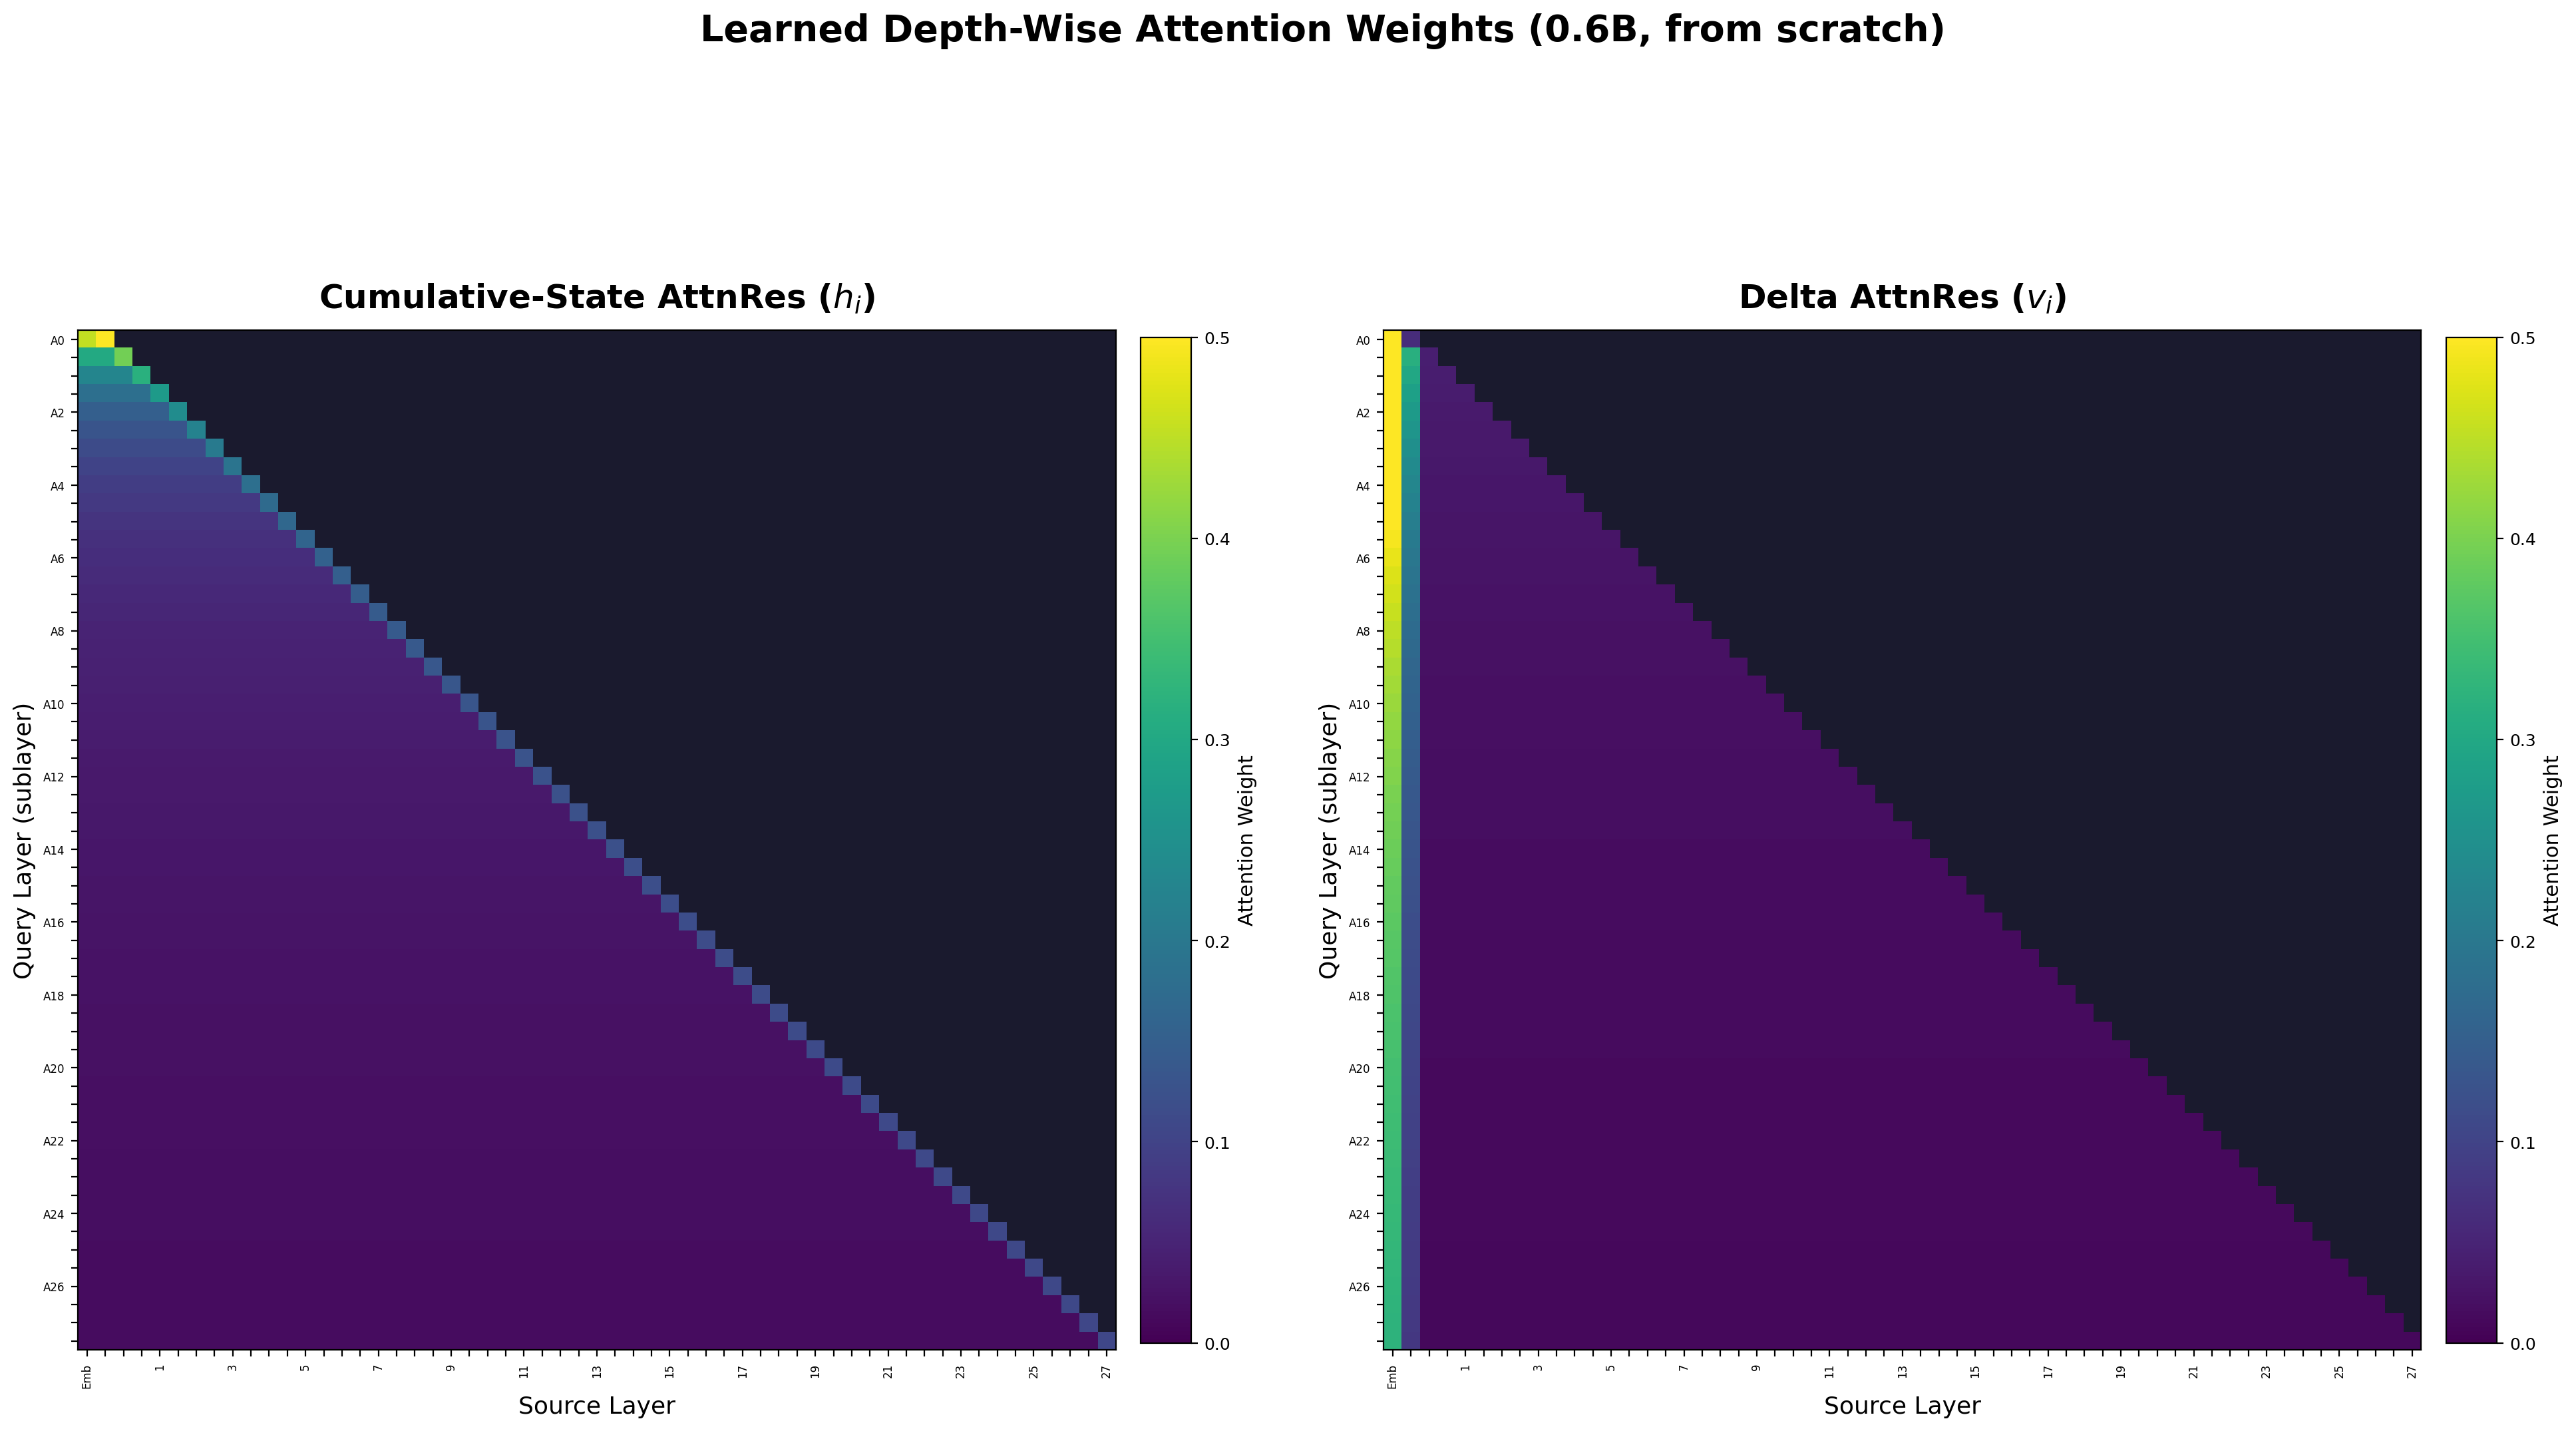
\includegraphics[width=\textwidth]{figures/fig2_routing_patterns.png}
\caption{\textbf{Learned attention weights.} \textbf{Left}: Cumulative-state AttnRes---attention is diffuse due to source redundancy. \textbf{Right}: Delta AttnRes---layers develop selective cross-layer shortcuts, with deep layers concentrating on early-layer outputs.}
\label{fig:routing}
\end{figure}

Delta AttnRes develops qualitatively different routing patterns from cumulative-state variants:
\begin{itemize}
    \item \textbf{Sharp routing}: Deep layers concentrate $>$50\% attention on specific early-layer outputs, forming learned cross-layer shortcuts.
    \item \textbf{Layer~0 prominence}: The embedding and first-layer outputs receive disproportionate attention from deep layers, consistent with the finding that early representations contain information progressively diluted by standard residual accumulation.
    \item \textbf{Alternating attention/MLP pattern}: The model distinguishes between attention and MLP outputs, selectively routing to the appropriate sublayer type.
\end{itemize}

\subsection{Training Dynamics}

The gated variants exhibit smoother optimization compared to ungated Delta AttnRes. At initialization ($w_l = 0$), the softmax gives uniform weights across all sources, and the model begins by averaging previous sublayer outputs equally. As training progresses, the queries specialize and routing patterns sharpen. This zero-init strategy is stable: the model transitions smoothly from uniform routing to selective shortcuts without loss spikes.

Block AttnRes achieves lower training loss because it operates over fewer, more distinctive sources---the softmax has an easier optimization landscape. However, the per-sublayer routing of Delta AttnRes provides finer-grained information retrieval that benefits downstream generalization.

Delta+Block AttnRes combines these advantages most effectively: it retains the compact 8-source optimization landscape of Block AttnRes while using delta representations that reduce source redundancy, achieving the lowest training loss (3.196) and the best evaluation across all metrics (WT2 PPL 43.22, 28\% below baseline).

%% ============================================================
\section{Related Work}
%% ============================================================

\paragraph{Cross-Layer Connections.} DenseNet~\citep{huang2017densely} concatenates all previous layer outputs. DenseFormer~\citep{pagliardini2024denseformer} introduces learned per-layer scalar weights but cannot be added post-hoc. Highway Networks~\citep{srivastava2015highway} and Hyper-Connections~\citep{zhu2024hyperconnections} use gating for layer-wise information flow. MUDDFormer~\citep{wang2024muddformer} generates position-dependent cross-layer weights via a small MLP and crucially decouples them across Q/K/V/residual streams, showing that per-stream routing improves over shared routing. Attention Residuals~\citep{kimi2025attention} use softmax attention over previous outputs, demonstrating improved scaling laws at up to 16B parameters. We extend this line of work in two ways: (1)~showing that source representation (delta vs.\ cumulative) is critical for effective routing, and (2)~introducing per-stream delta routing that achieves MUDDFormer-style stream decoupling within the attention-based routing framework, with $10\times$ fewer additional parameters and fully interpretable routing weights.

\paragraph{Residual Stream Analysis.} \citet{veit2016residual} show that residual networks behave like ensembles of shallow networks, and \citet{elhage2021mathematical} formalize the ``residual stream'' view where each layer reads from and writes to a shared state. \citet{clark2019bert} analyze attention patterns across layers, finding that different heads specialize in different linguistic relations. Our work is complementary: we show that the \emph{source representation} of cross-layer attention determines whether the model can learn such specialization---cumulative states collapse this capacity while delta sources preserve it.

\paragraph{Gating Mechanisms.} GLU variants~\citep{shazeer2020glu} apply gating within feed-forward layers. Gated attention~\citep{qiu2025gated} applies sigmoid gates to attention values. ReZero~\citep{bachlechner2020rezero} initializes residual branches with zero scalars for stable deep training. Mixture-of-Experts~\citep{shazeer2017moe,fedus2022switch} use sparse gating to route tokens to specialized experts.

\paragraph{Scaling Laws.} \citet{kaplan2020scaling} and \citet{hoffmann2022chinchilla} establish scaling laws for language models relating compute, data, and model size. Attention Residuals~\citep{kimi2025attention} demonstrate improved scaling exponents with cross-layer routing. Our Delta formulation should further improve these scaling properties by enabling more effective routing, though we leave scaling law experiments beyond 1.7B to future work.

%% ============================================================
\section{Conclusion}
%% ============================================================

We demonstrate that the source representation is a critical and previously underexplored design choice in Attention Residuals. Delta sources---per-sublayer outputs rather than cumulative hidden states---avoid the source redundancy problem that plagues cumulative implementations, enabling effective softmax routing with sharp, meaningful cross-layer shortcuts.

Our findings:
\begin{enumerate}
    \item \textbf{What to route matters most}: Cumulative states have 0.95 cosine similarity, collapsing softmax to near-uniform. Delta sources are naturally distinctive, providing 7.5--19.2\% PPL reduction.
    \item \textbf{Where to route provides complementary gains}: Per-stream V-routing improves results on top of both cumulative and delta sources. The two dimensions are orthogonal and compose nearly additively.
    \item \textbf{Delta + per-stream V is optimal}: Combining delta sources with V-routing achieves the best results across all configurations tested (nanoGPT, Qwen3 100M--0.6B).
    \item \textbf{Additive routing enables fine-tuning}: Delta AttnRes's additive formulation preserves the residual stream at initialization, achieving 29.2\% PPL reduction when fine-tuning Qwen3-0.6B.
    \item \textbf{Minimal overhead}: 0.034\% additional parameters (with per-stream routing) and $<$1\% compute overhead, making Delta-V AttnRes a practical drop-in improvement for any transformer.
\end{enumerate}

Code, pretrained weights, and visualization tools are available at \url{https://github.com/wdlctc/open-attention-residuals}.

\bibliographystyle{plainnat}
\bibliography{references}

\newpage
\appendix

%% ============================================================
\section{Original Block Attention Residuals: Implementation}
\label{app:block_attnres}
%% ============================================================

We reproduce below the PyTorch-style pseudo code for Block Attention Residuals from \citet{kimi2025attention}, followed by a side-by-side comparison with our Delta formulation.

\begin{figure}[h]
\begin{lstlisting}[style=python]
def block_attn_res(blocks: list[Tensor], partial_block: Tensor,
                   proj: Linear, norm: RMSNorm) -> Tensor:
    """
    Inter-block attention: attend over block reps + partial sum.
    blocks:
        N tensors of shape [B, T, D]: completed block representations
        for each previous block
    partial_block:
        [B, T, D]: intra-block partial sum (b_n^i)
    """
    V = torch.stack(blocks + [partial_block])  # [N+1, B, T, D]
    K = norm(V)
    logits = torch.einsum('d, n b t d -> n b t', proj.weight.squeeze(), K)
    h = torch.einsum('n b t, n b t d -> b t d', logits.softmax(0), V)
    return h

def forward(self, blocks: list[Tensor], hidden_states: Tensor
           ) -> tuple[list[Tensor], Tensor]:
    partial_block = hidden_states
    # apply block attnres before attn
    # blocks already include token embedding
    h = block_attn_res(blocks, partial_block,
                       self.attn_res_proj, self.attn_res_norm)

    # if reaches block boundary, start new block
    # block_size counts ATTN + MLP; each transformer layer has 2
    if self.layer_number % (self.block_size // 2) == 0:
        blocks.append(partial_block)
        partial_block = None

    # self-attention layer
    attn_out = self.attn(self.attn_norm(h))
    partial_block = partial_block + attn_out if partial_block is not None else attn_out

    # apply block attnres before MLP
    h = block_attn_res(blocks, partial_block,
                       self.mlp_res_proj, self.mlp_res_norm)

    # MLP layer
    mlp_out = self.mlp(self.mlp_norm(h))
    partial_block = partial_block + mlp_out

    return blocks, partial_block
\end{lstlisting}
\caption{PyTorch-style pseudo code for Block Attention Residuals~\citep{kimi2025attention}. \texttt{block\_attn\_res} computes softmax attention over block representations using a learned pseudo-query $w_l$; \texttt{forward} is a single-layer pass that maintains \texttt{partial\_block} ($b_n^i$, intra-block residual) and \texttt{blocks} ($[b_0, \ldots, b_{n-1}]$, inter-block history).}
\label{fig:block_code}
\end{figure}

\subsection{Key Differences from Delta AttnRes}

Table~\ref{tab:diff} summarizes the implementation differences between Block AttnRes and our Delta AttnRes (Figure~\ref{fig:delta_code}).

\begin{table}[h]
\centering
\caption{Implementation comparison: Block AttnRes vs.\ Delta AttnRes.}
\label{tab:diff}
\begin{tabular}{lll}
\toprule
\textbf{Aspect} & \textbf{Block AttnRes} & \textbf{Delta AttnRes (ours)} \\
\midrule
Source type & Cumulative partial sums $b_n^i$ & Individual sublayer outputs $v_i$ \\
What is stored & \texttt{partial\_block} (cumul.) & \texttt{attn\_out}, \texttt{mlp\_out} (deltas) \\
When stored & Block boundaries only & Every sublayer \\
Num.\ sources ($L{=}28$) & $N{=}8$ blocks & $2L{=}56$ sublayer outputs \\
Source diversity & Low (adj.\ cos sim 0.95) & High (adj.\ cos sim $<$0.3) \\
Routing function input & \texttt{blocks + [partial\_block]} & \texttt{deltas} \\
Routing function output & $h = \sum \alpha_i s_i$ (replace) & $h = \tilde{h} + \sum \alpha_i v_i$ (additive) \\
Memory & $O(N \cdot T \cdot d)$ & $O(2L \cdot T \cdot d)$ \\
\bottomrule
\end{tabular}
\end{table}

The most important distinction is \emph{semantic}: Block AttnRes sources are cumulative states that represent ``everything computed up to block $n$'', while Delta AttnRes sources are incremental contributions that represent ``what sublayer $i$ specifically added.'' The former leads to high inter-source redundancy (adjacent cumulative states differ by only $v_i \ll h_i$); the latter preserves the natural diversity between attention and MLP computations across different depths.

A secondary difference is \emph{structural}: Block AttnRes computes $h = \sum \alpha_i s_i$ as a \emph{replacement} for the residual stream, while Delta AttnRes computes $h = \tilde{h} + \sum \alpha_i v_i$ as an \emph{additive} correction. At initialization ($w_l = 0$), Block AttnRes returns the uniform average of all sources (disrupting the residual stream), while Delta AttnRes adds the uniform average of all deltas to the existing residual stream (a smaller perturbation since $\|v_i\| \ll \|h_i\|$).

\end{document}
